\documentclass{article}

\usepackage{hyperref}
\usepackage[table]{xcolor}
\usepackage{graphicx}
\graphicspath{{images/}}

\begin{document}

\begin{titlepage}

\title{r32 CPU and Instruction Set}
\author{Reed Foster}
\date{June 2017}
\maketitle
\thispagestyle{empty}

\end{titlepage}

\pagenumbering{roman}
\tableofcontents

\newpage

\section*{About r32}
\addcontentsline{toc}{section}{About r32}
r32 is a fully-fledged, 32-bit microcontroller/SoC with a CPU-core based on the MIPS architecture.
\subsection*{Architecture}

\begin{figure}[h]
\caption{r32 Block Diagram}
\label{fig:r32blockdiagram}
\centering
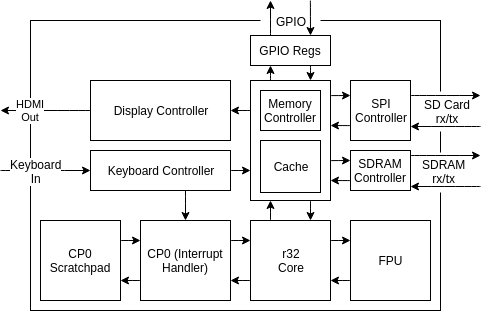
\includegraphics[scale=0.7]{architecture.png}
\end{figure}

\newpage

\pagenumbering{arabic}
\setcounter{page}{1}

\section{Instruction Set}
The r32 core instruction set is based on MIPS, an instruction set developed MIPS Technologies (founded by researchers from Stanford University). MIPS is a RISC architecture, with a 5-stage pipeline and 128-byte register file. r32's instruction set is mostly a subset of MIPS, with a few tweaks to the programmer's interface to the processor.

\subsection{Instruction Format}

\subsection{Processor Instructions}

\begin{table}[h]

\centering
\begin{tabular}{c c c}

\centering
\definecolor{light-gray}{gray}{0.8}
\rowcolors{1}{white}{light-gray}
\begin{tabular}[t]{| c | c | c |}
\hline
\multicolumn{3}{| c |}{CPU Core} \\
\hline
add     & addi & addiu \\
addu    & and  & andi  \\
beq     & bgez & bgtz  \\
blez    & bltz & bne   \\
j       & jr   & lb    \\
lbu     & lh   & lhu   \\
lui     & lw   & nor   \\
or      & ori  & pre   \\
sub     & sh   & sll   \\
sllv    & slt  & slti  \\
sltiu   & sltu & sra   \\
srav    & srl  & srlv  \\
sub     & subu & sw    \\
syscall & teq  & teqi  \\
tge     & tgei & tgeiu \\
tgeu    & tlt  & tlti  \\
tltiu   & tltu & tne   \\
tnei    & xor  & xori  \\
\hline
\end{tabular}

\centering
\definecolor{light-gray}{gray}{0.8}
\rowcolors{1}{white}{light-gray}
\begin{tabular}[t]{| c | c |}
\hline
\multicolumn{2}{| c |}{CP0} \\
\hline
lwc0 & mfc0 \\
mtc0 & swc0 \\
\hline
\end{tabular}

\centering
\definecolor{light-gray}{gray}{0.8}
\rowcolors{1}{white}{light-gray}
\begin{tabular}[t]{| c | c | c |}
\hline
\multicolumn{3}{| c |}{CP1 (FPU)} \\
\hline
bc1f & bc1t  & ceq  \\
cfc1 & cge   & cgt  \\
cle  & clt   & cne  \\
ctc1 & fabs  & fadd \\
fdiv & fma   & fmul \\
fneg & fsqrt & fsub \\
lwc1 & mfc1  & mov  \\
mtc1 & swc1  &      \\
\hline
\end{tabular}

\end{tabular}
\caption{Supported processor and coprocessor instructions}
\label{tab:processorinstructions}
\end{table}

\section{Memory}
Memory information

\subsection{SDRAM}
\subsubsection{What is SDRAM?}
SDRAM stands for Synchronous DRAM, or Synchronous Dynamic Random Access Memory. SRAM, or Static Random Access Memory, the fast style of memory found in cache memory on the CPU die, is made up of transistors that form a circuit that has similar behavior to a latch or flip-flop. DRAM and SDRAM, however, use small capacitors to store each bit, and as a result, DRAM-style memories are much cheaper per byte than SRAM. Because DRAM uses capacitors to store data, each bit must be refreshed frequently to maintain its state. Fortunately, SDRAM modules have control circuitry that automates a lot of the maintainance tasks surrounding DRAM, so memory controllers that interface with SDRAM aren't as difficult to design. That being said, SDRAM presents a far more complex interface than SRAM.

\subsubsection{Why Build an SDRAM Controller?}
The FPGA development board that I own, the miniSpartan6+, comes with a 16Mx16bit (256Mb, 32MB) DDR SDRAM chip (presumably SDRAM was chosen to provide a large memory and keep the cost of the board down). In my $\mu$CPU project, I used distributed RAM in the FPGA, which used up a large amount of resources. I hoped to write an SDRAM controller for that project, but never got around to it. In this project, the SDRAM controller increases memory capacity and frees up logic elements for computational tasks.

\subsubsection{First Steps}
In order to write a controller for a peripheral device, I need to understand very well both the operation of the intended device as well as the protocol required to communicate with it. Starting this project, all I knew about SDRAM was what the acronym stood for along with the fact that it uses capacitors instead of transistors to store data. One of the first confusing things for me was how the chip I was using could have 16M addresses but only a 13-bit address ($2^{13} = 8192$ or $8K$). It was then that I realized how different SDRAM is from SRAM. In order to access a word of data in SDRAM, one must first activate a row in a bank (supplying what constitutes a 15-bit address in my case, 2-bit bank $+$ 13 bit row address), and then supply a 9-bit column address when reading. This totals to 24 bits of address, which makes sense because $2^{24} = 16M$. One of the neat things about SDRAM that allows it to perform very well despite the large latencies reads experience at high clock frequencies is its capability to burst. The particular SDRAM I am using allows for 1-word, 2-word, 4-word, 8-word, and full-page (512-word) bursts. Because I plan on using a caching hierarchy on the FPGA, I opted for the 512-word burst because it will allow me maximum bandwith, and I only need to read/write to memory when a cache miss occurs.This simplifies the SDRAM controller a lot because I don't have to add optimization logic to group requests for addresses in the same bank/row.

\subsubsection{Other Projects}
I'm certainly not the first one to design an SDRAM controller in VHDL to run on an FPGA. As such, there are tons (not that many, but a lot) of SDRAM controllers out there, some of which would probably work on my board with not too much tweaking. However, as I intend to build the whole CPU-core and its peripheral interfaces from scratch, I opted to use others designs purely as reference and learning material. I most heavily relied on Mike Field's two SDRAM controllers (\href{http://hamsterworks.co.nz/mediawiki/index.php/SDRAM_Memory_Controller}{complex one} and \href{http://hamsterworks.co.nz/mediawiki/index.php/Simple_SDRAM_Controller}{simpler one}), and obviously, the datasheet of the part I am using.

\subsubsection{Finite State Machine}
At the heart of the SDRAM controller is a Finite State Machine, or FSM. As always, before I started writing VHDL, I created a diagram in order to more easily translate my ideas to code. Figure \ref{fig:sdramfsm} shows the 2nd (current) revision of the SDRAM state machine used to drive the controller. The green states indicate states in which data is being transferred (read/written) There are a lot of different states in this diagram because when I designed it, I wanted the logic for transitioning between states to be very simple and only require a few timers. First, the SDRAM is initialized (blue states). The datasheet for the SDRAM chip specifies a 200$\mu$s startup where all control signals must be held constant. This is achieved by using a counter that counts from $200,000 / t_{ck}$ to 0 where $t_{ck}$ is the period of the clock (ns). The rest of the delays are implemented the same way. The loopback state transitions labeled $t_{rp}$, $t_{mrd}$, $t_{rp}$, etc. are timing constraints specified in the SDRAM datasheet.

\begin{figure}[!htb]
\caption{SDRAM Finite State Machine}
\label{fig:sdramfsm}
\centering
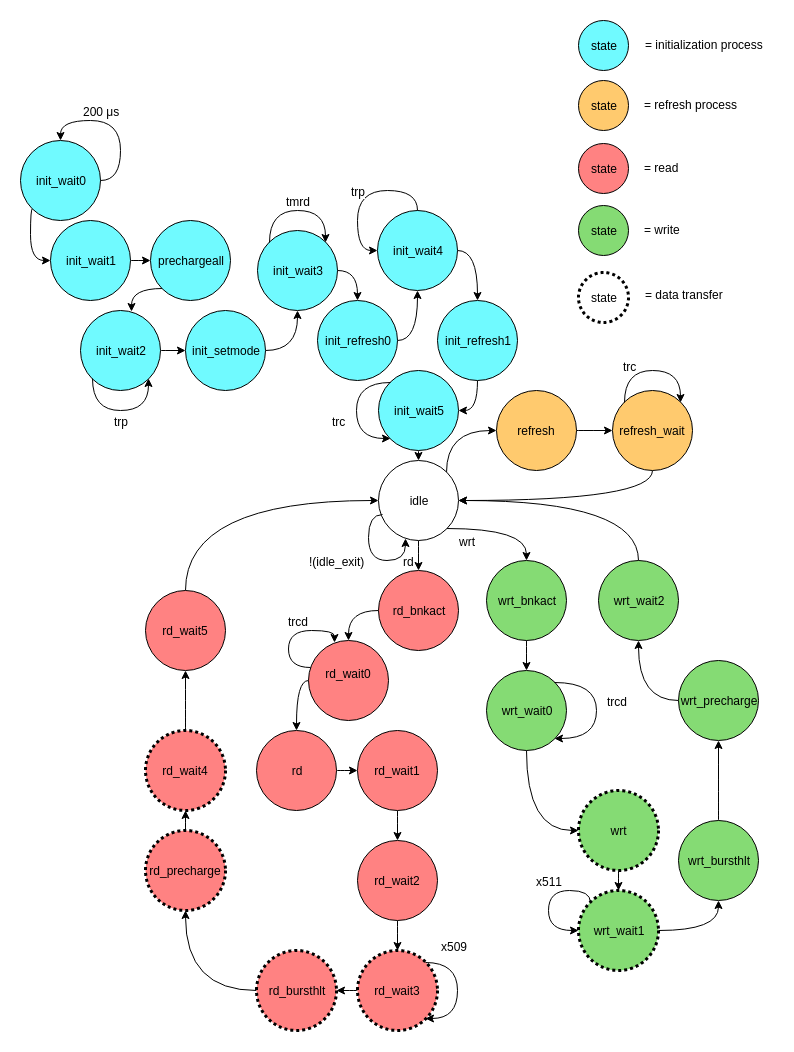
\includegraphics[scale=0.23]{sdramfsm2.png}
\end{figure}

\newpage

\subsubsection{FIFOs}
In order to maximize cache efficiency, I have added FIFO queues to the data input and output on the SDRAM controller. This allows the cache to quickly free up a line that has old data in it by writing the evicted data to a buffer without waiting for the controller to be ready to write. The FIFO on the output of the controller achieves a similar goal, alllowing the SDRAM controller to read from the SDRAM uninterrupted and write all of the read data to the buffer. In addition to buffering data, I also use a small FIFO as a "request" queue. This allows the CPU cache logic to make requests to read or write to SDRAM, even if the SDRAM controller is currently accessing the SDRAM. The CPU cache can request to write data and begin to write data into the transmit FIFO while the SDRAM controller is still busy processing a previous read or write request, and then proceed to manage the cache until it the data is ready. Originally, all FIFO queues were synchronous, with a single clock for both enqueue and dequeue operations. However, I decided that in order to test that the burst was working properly, I should add dual-clock or asynchronous FIFOs so that I can read data out very slowly (i.e. a human can see the contents of each memory location with 8 leds) from the data out queue.

\newpage

\section{I/O}
I/O information
\end{document}